Prior to using a one-dimensional phononic bandgap on our high-stress silicon nitride (\ce{Si3N4}) membrane sample, we used commercial fabricated Norcada \ce{Si3N4} membranes\footnote{\url{http://www.norcada.com/products/high-q-si3n4-membrane/}}. However, they suffered greatly from reduction of quality factor $Q$ when clamped \cite{wilson2009}. The overall goal is to have a quantum enabled system and that means for most experiments, i.e. squeezing \cite{purdy2013} and ground state cooling \cite{chan2011}, cryogenically pre-cooling the membrane as much as possible, before starting the experiments. This is due to the fact that our final phonon occupancy is proportional to the bath temperature as shown in equation \eqref{eq:nf}. This requires clamping of the sample to achieve good thermal flow from the cold finger to the sampler holder and into the sample. At the same time we do not want to compromise the $Q$'s in order to do so. Luckily the idea of membrane shielding by a phononic bandgap was proposed \cite{tsaturyan2014, yu2014} and fabricating them is a huge step in the right direction for the membrane-in-middle optomechanical system. A picture of such a membrane is shown in figure \ref{fig:sample}. For insight into fabrication processes see \cite{tsaturyan2014}.

\begin{figure}[H]
\centering
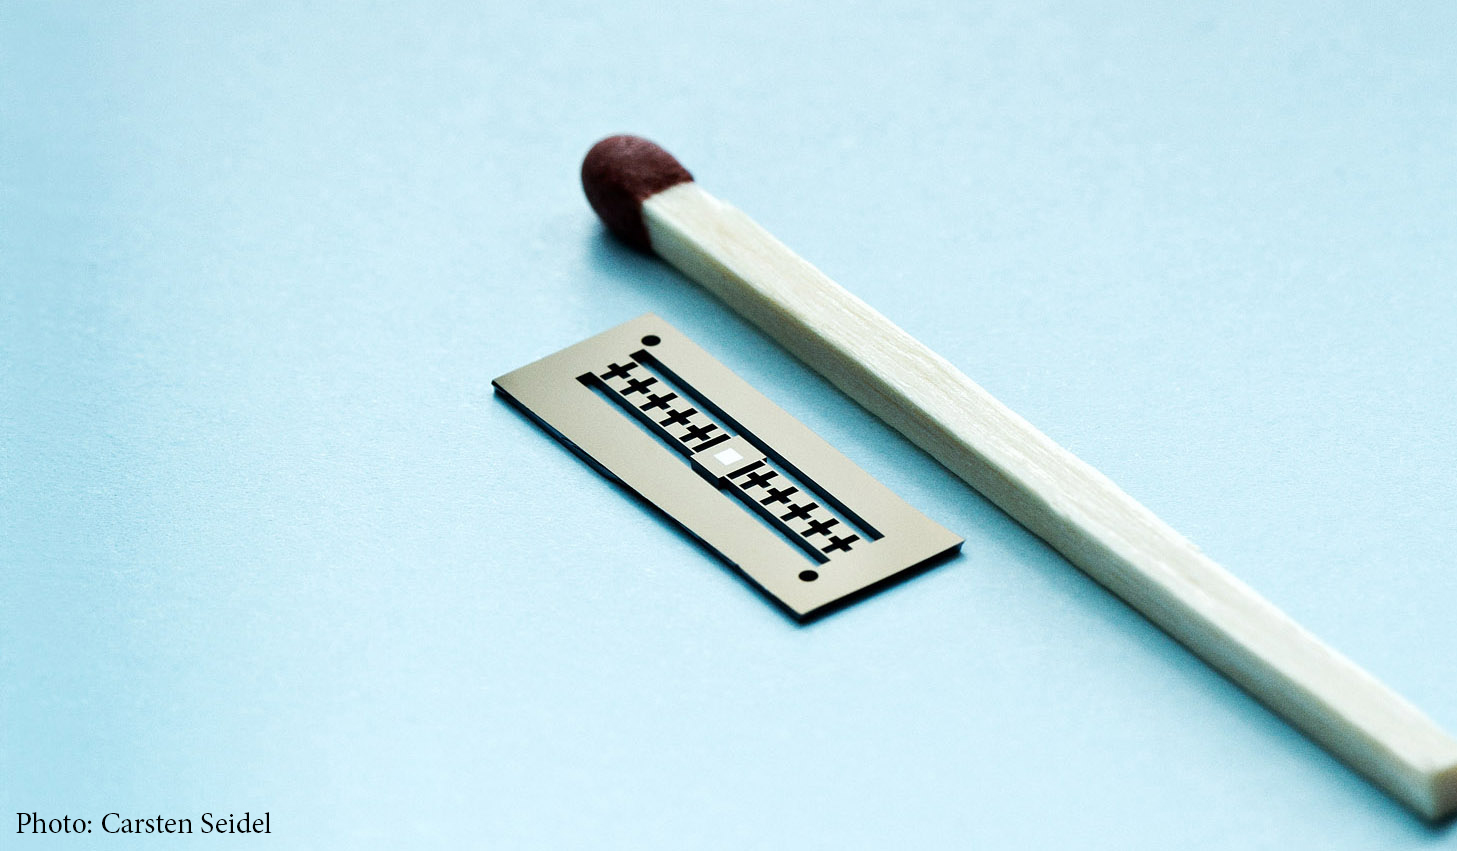
\includegraphics[scale=0.25]{Seidel_02.jpg}
\caption{Silicon nitride membrane shielded by a one-dimensional phononic bandgap next to a match for size comparison.}
\label{fig:sample}
\end{figure}

A problem with this generation of samples, is the low fundamental frequency ($\sim$\SI{13}{\kilo\hertz})\cite{tsaturyan2014} of the phononic bridge, on which the membrane is suspended on. Due to the low frequency of the bridge mode, there is significant excitaions from the surrounding environment. This makes locking the laser to the cavity resonance with high input powers very challenging. Therefore, in this work we were forced to dampen the bridge by placing chips with no suspended membranes on both sides of the actual test sample, thus disabling the effect of the phononic shield.

As a small side remark we also make spacers for the cavity assembly, which is done breaking of the phononic bridge of a normal chip. Since the surface of the silicon is extremely smooth, they make a good spacer, as will be evident in the section below.